\section{Auswertung}
Die in der Auswertung bestimmten Ausgleichsrechnungen werden mit
dem Python Paket \emph{scipy.optimize}\cite{scipy} durchgeführt.
Des Weiteren werden die Fehler und insbesondere die Fehlerfortpflanzungen
mit dem Python Paket \emph{uncertainties}\cite{uncertainties} berechnet.
Zusätzlich werden die benötigten Naturkonstanten dem Python Paket \emph{scipy.constants}\cite{scipy.constants}
entommen.

\subsection{Untersuchung der Bragg-Bedingung}
Die an der Messapperatur eingestellten Konfiguration lauten:
\begin{equation*}
  \theta=\SI{14}{\degree}, \quad \alpha\ua{GM}\in\left[26,30\right]\,\si{\degree},\quad \Delta\alpha\ua{GM}=\SI{0.1}{\degree}, \quad \Delta t=\SI{10}{\second}.
\end{equation*}
Eine Liste mit den gemessenen Werten ist in Tabelle \ref{tab: bragg_test} zu finden und in Abbildung \ref{fig: bragg_plot} abgebildet.
\begin{table} 
\centering 
\caption{Messwerte bei der Untersuchung der Bragg Bedingung.} 
\label{tab: bragg_test} 
\begin{tabular}{S S S S } 
\toprule  
{$\alpha_{\mathrm{Gl}} \, / \, \si{\degree}$} & {$I \, / \, \mathrm{Imp}/\mathrm{s}$} & {$\alpha_{\mathrm{Gl}} \, / \, \si{\degree}$} & {$I \, / \, \mathrm{Imp}/\mathrm{s}$}  \\ 
\midrule  
 26.0  & 41  & 28.1  & 156\\ 
26.1  & 41  & 28.2  & 158\\ 
26.2  & 44  & 28.3  & 165\\ 
26.3  & 43  & 28.4  & 168\\ 
26.4  & 47  & 28.5  & 169\\ 
26.5  & 47  & 28.6  & 156\\ 
26.6  & 53  & 28.7  & 148\\ 
26.7  & 56  & 28.8  & 137\\ 
26.8  & 68  & 28.9  & 125\\ 
26.9  & 75  & 29.0  & 119\\ 
27.0  & 73  & 29.1  & 110\\ 
27.1  & 83  & 29.2  & 105\\ 
27.2  & 91  & 29.3  & 91\\ 
27.3  & 102  & 29.4  & 86\\ 
27.4  & 110  & 29.5  & 69\\ 
27.5  & 122  & 29.6  & 66\\ 
27.6  & 118  & 29.7  & 53\\ 
27.7  & 133  & 29.8  & 43\\ 
27.8  & 140  & 29.9  & 40\\ 
27.9  & 150  & 30.0  & 40\\ 
\bottomrule 
\end{tabular} 
\end{table}
\begin{figure}
  \centering
  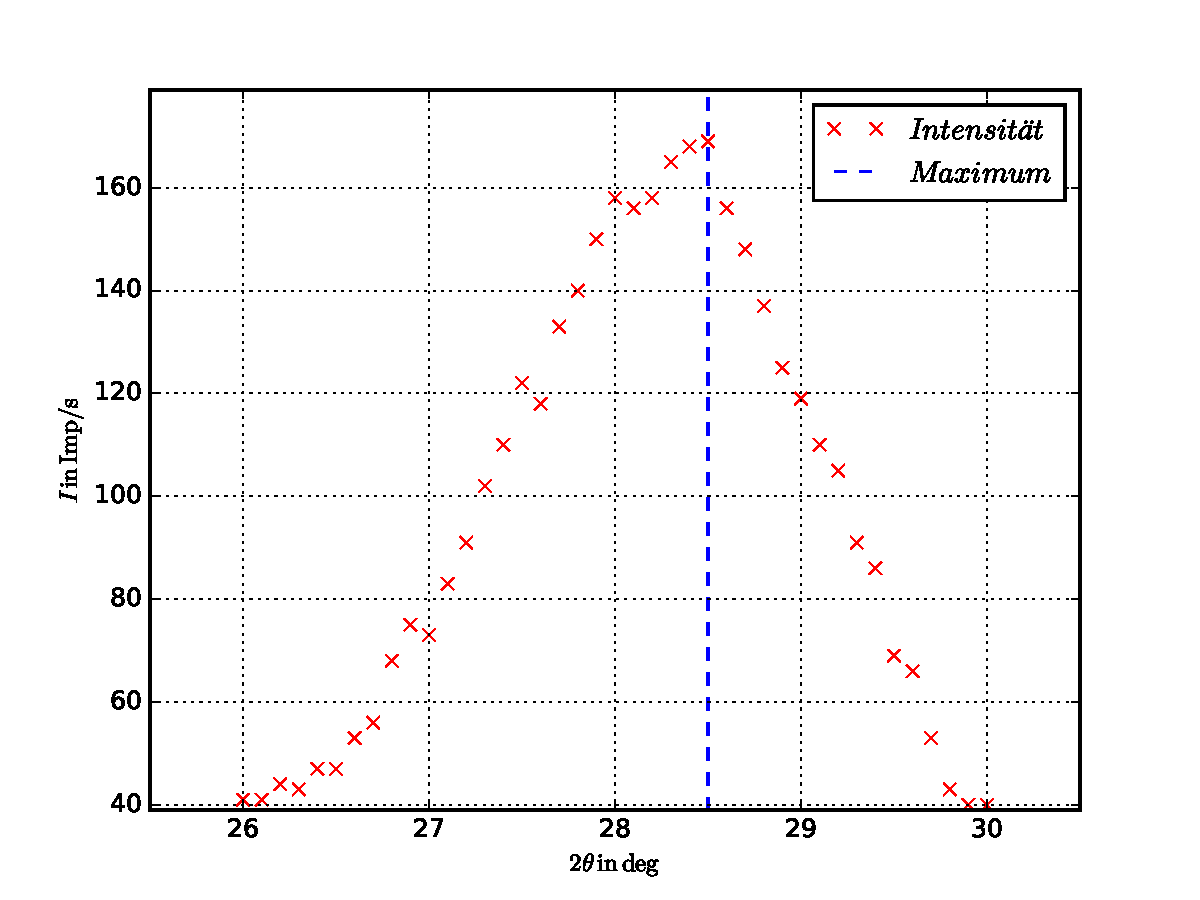
\includegraphics[width=0.8 \textwidth]{../Messdaten/bragbed.pdf}
  \caption{Messwerte zur Untersuchung der Bragg-Bedingung.} %Hingegen passt nicht
  \label{fig: bragg_plot}
\end{figure}
Das Maximum der Messwerte ist der bestimmte Bragg-Winkel:
\begin{equation}
  \label{eq:bestimmt_bragg_winkel}
  2\theta\ua{bragg}=\SI{28.5}{\degree} \quad \Leftrightarrow \quad \theta\ua{bragg}=\SI{14.25}{\degree}.
\end{equation}

\subsection{Untersuchung des Emissionspektrum von $\ce{Cu}$}
Zu Beginn wird der $2:1$ Kopplungsmodus der Apperatur gewählt und folgende Parameter eingestellt:
\begin{equation*}
  \theta\in\left[4,26\right]\,\si{\degree},\quad \Delta\theta=\SI{0.2}{\degree}, \quad \Delta t=\SI{5}{\second}.
\end{equation*}
Die aufgenommen Werte sind in Tabelle \ref{tab: emi_cu} aufgelistet und in Abbildung \ref{fig: emission_cu} dargestellt.
\begin{table} 
\centering 
\caption{Messwerte bei der Untersuchung des Emmissionspektrum von $\ce{Cu}$.} 
\label{tab: emi_cu} 
\begin{tabular}{S S } 
\toprule  
{$\theta \, / \, \si{\degree}$} & {$I \, / \, \mathrm{Imp}/\mathrm{s}$}  \\ 
\midrule  
 4.0  & 30.0\\ 
4.2  & 27.0\\ 
4.4  & 29.0\\ 
4.6  & 31.0\\ 
4.8  & 34.0\\ 
5.0  & 43.0\\ 
5.2  & 51.0\\ 
5.4  & 61.0\\ 
5.6  & 64.0\\ 
5.8  & 67.0\\ 
6.0  & 83.0\\ 
6.2  & 87.0\\ 
6.4  & 94.0\\ 
6.6  & 104.0\\ 
6.8  & 118.0\\ 
7.0  & 128.0\\ 
7.2  & 127.0\\ 
7.4  & 145.0\\ 
7.6  & 145.0\\ 
7.8  & 159.0\\ 
8.0  & 156.0\\ 
8.2  & 169.0\\ 
8.3  & 168.0\\ 
8.6  & 178.0\\ 
8.8  & 181.0\\ 
9.0  & 188.0\\ 
9.2  & 185.0\\ 
9.3  & 204.0\\ 
9.6  & 204.0\\ 
9.8  & 198.0\\ 
10.0  & 215.0\\ 
10.2  & 211.0\\ 
10.4  & 225.0\\ 
10.6  & 231.0\\ 
10.8  & 211.0\\ 
11.0  & 235.0\\ 
11.2  & 221.0\\ 
11.4  & 215.0\\ 
11.6  & 218.0\\ 
11.8  & 201.0\\ 
12.0  & 225.0\\ 
12.2  & 220.0\\ 
12.4  & 212.0\\ 
12.6  & 220.0\\ 
12.8  & 195.0\\ 
13.0  & 175.0\\ 
13.2  & 166.0\\ 
13.4  & 176.0\\ 
13.6  & 163.0\\ 
13.8  & 162.0\\ 
14.0  & 163.0\\ 
14.2  & 161.0\\ 
14.4  & 154.0\\ 
14.6  & 153.0\\ 
14.8  & 151.0\\ 
15.0  & 150.0\\ 
15.2  & 145.0\\ 
15.4  & 146.0\\ 
15.6  & 136.0\\ 
15.8  & 137.0\\ 
16.0  & 140.0\\ 
16.2  & 130.0\\ 
16.4  & 130.0\\ 
16.6  & 117.0\\ 
16.8  & 122.0\\ 
17.0  & 126.0\\ 
17.2  & 114.0\\ 
17.4  & 118.0\\ 
17.6  & 105.0\\ 
17.8  & 119.0\\ 
18.0  & 98.0\\ 
18.2  & 110.0\\ 
18.4  & 104.0\\ 
18.6  & 112.0\\ 
18.8  & 119.0\\ 
19.0  & 101.0\\ 
19.2  & 110.0\\ 
19.4  & 121.0\\ 
19.6  & 464.0\\ 
19.8  & 1194.0\\ 
20.0  & 761.0\\ 
20.2  & 169.0\\ 
20.4  & 147.0\\ 
20.6  & 123.0\\ 
20.8  & 120.0\\ 
21.0  & 116.0\\ 
21.2  & 113.0\\ 
21.4  & 122.0\\ 
21.6  & 165.0\\ 
21.8  & 316.0\\ 
22.0  & 4140.0\\ 
22.2  & 3604.0\\ 
22.4  & 333.0\\ 
22.6  & 144.0\\ 
22.8  & 110.0\\ 
23.0  & 92.0\\ 
23.2  & 86.0\\ 
23.4  & 83.0\\ 
23.6  & 67.0\\ 
23.8  & 75.0\\ 
24.0  & 69.0\\ 
24.2  & 67.0\\ 
24.4  & 64.0\\ 
24.6  & 61.0\\ 
24.8  & 60.0\\ 
25.0  & 58.0\\ 
25.2  & 0.0\\ 
25.4  & 54.0\\ 
25.6  & 55.0\\ 
25.8  & 48.0\\ 
26.0  & 45.0\\ 
\bottomrule 
\end{tabular} 
\end{table}
\begin{figure}
  \centering
  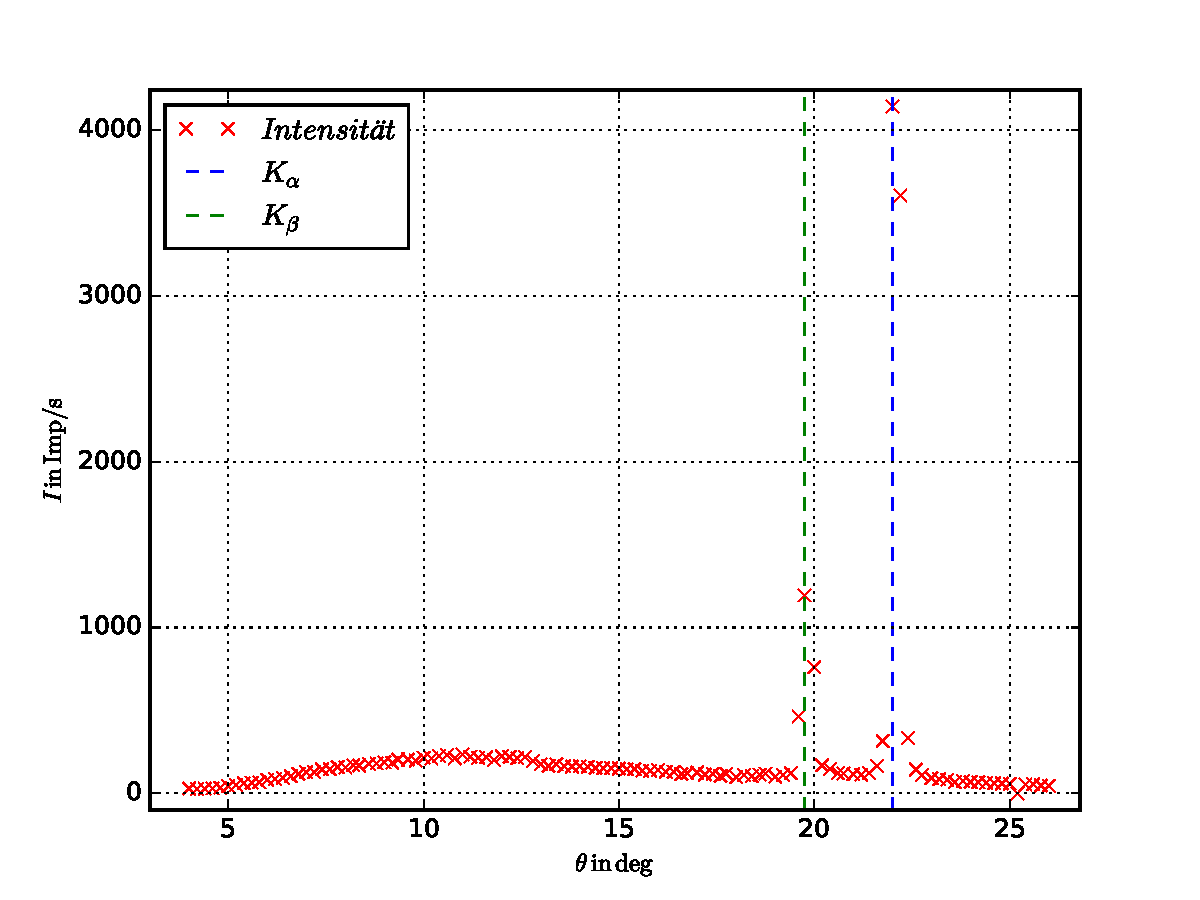
\includegraphics[width=0.8 \textwidth]{../Messdaten/emission_cu.pdf}
  \caption{Messsung des Emmissionspektrums von $\ce{Cu}$.} %Hingegen passt nicht
  \label{fig: emission_cu}
\end{figure}
In der Abbildung sind die $K_\alpha$ und $K_\beta$ Kante mit eingezeichnet.
Aus dem Experiment ergebens sich die folgenden Werte:
\begin{equation}
  \label{eq:k_alpha,k_beta}
  K_\alpha=\SI{8.2}{\kilo\eV} \qquad   K_\beta=\SI{9.1}{\kilo\eV}.
\end{equation}
Die maximale Energie beläuft sich auf:
\begin{equation}
  \label{eq: maximale_energie}
  E\ua{max}=\SI{44.1}{\kilo\eV}
\end{equation}
Die Winkel werden dabei mit Gleichung \eqref{} umgerechnet.
Mit Hilfe der Energien \eqref{eq:k_alpha,k_beta}, können die Abschirmkonstanten
für die einzelnen K- Linien bestimmt werden.
Aus den Formeln \eqref{} errechnet sich:
\begin{equation}
   \label{eq:abschirm}
   \sigma_1=3.13 \qquad \sigma_2=20.9.
\end{equation}

\textbf{Es fehlt noch die Halbwertsbreite}

\subsection{Analyse von Absorptionsspektren}

Die im $2:1$ Kopplungsmodus betriebene Versuchsapperatur wurde wie folgt eingestellt:
\begin{equation*}
  \theta\in\left[\theta\ua{K}-2,\theta\ua{K}+2\right]\,\si{\degree},\quad \Delta\theta=\SI{0.1}{\degree}, \quad \Delta t=\SI{20}{\second}.
\end{equation*}
Der Winkel $\theta\ua{K}$ ist der Winkel an für die Probe das Maximum erwartet
wird. Die Liste mit allen zu untersuchenden Materialen und Winkel ist in Tabelle
\ref{tab: theta_k} zu finden.
\begin{table}
  \centering
  \caption{Untersuchte Elemente und deren Grenzwinkel $\theta\ua{K,lit}$\cite{}.}
  \label{tab: theta_k}
  \begin{tabular}{S S S}
    \toprule
    {Element}& {$Z$} & {$\theta\ua{K,lit}$} \\
    \midrule
    $\ce{Zn}$& 30  & 9.65 \\
    $\ce{Zr}$&40 & 9.85 \\
    $\ce{Ge}$&32 & 17.3 \\
    $\ce{Br}$&35 & 13.2 \\
    $\ce{Sr}$&38 & 11.0 \\
    \bottomrule
  \end{tabular}
\end{table}
\subsubsection{Untersuchung von Zink $\ce{Zn}$}\label{sec: zink}
Die bei Zink gemessenen Werte sind in Tabelle \ref{tab: zink} aufgeführt.
\begin{table} 
\centering 
\caption{Messwerte bei der Untersuchung des Emmissionspektrum von $\ce{Cu}$.} 
\label{tab: zink} 
\begin{tabular}{S S } 
\toprule  
{$\theta \, / \, \si{\degree}$} & {$I \, / \, \mathrm{Imp}/\mathrm{s}$}  \\ 
\midrule  
 17.0  & 43.0\\ 
17.1  & 46.0\\ 
17.2  & 45.0\\ 
17.2  & 47.0\\ 
17.4  & 45.0\\ 
17.5  & 44.0\\ 
17.6  & 43.0\\ 
17.7  & 43.0\\ 
17.8  & 40.0\\ 
17.9  & 44.0\\ 
18.0  & 41.0\\ 
18.1  & 53.0\\ 
18.2  & 59.0\\ 
18.2  & 68.0\\ 
18.4  & 74.0\\ 
18.5  & 70.0\\ 
18.6  & 72.0\\ 
18.7  & 74.0\\ 
18.8  & 77.0\\ 
18.9  & 68.0\\ 
19.0  & 70.0\\ 
19.1  & 69.0\\ 
19.2  & 71.0\\ 
19.2  & 71.0\\ 
19.4  & 80.0\\ 
19.5  & 115.0\\ 
19.6  & 396.0\\ 
19.7  & 747.0\\ 
19.8  & 794.0\\ 
19.9  & 753.0\\ 
20.0  & 457.0\\ 
20.1  & 138.0\\ 
20.2  & 104.0\\ 
20.2  & 96.0\\ 
20.4  & 89.0\\ 
20.5  & 81.0\\ 
20.6  & 76.0\\ 
20.7  & 77.0\\ 
20.8  & 76.0\\ 
20.9  & 72.0\\ 
21.0  & 71.0\\ 
\bottomrule 
\end{tabular} 
\end{table}
In der Abbildung \ref{fig: absotp_zink} befindet sich die graphische Abbildung der Messdaten.
\begin{figure}
  \centering
  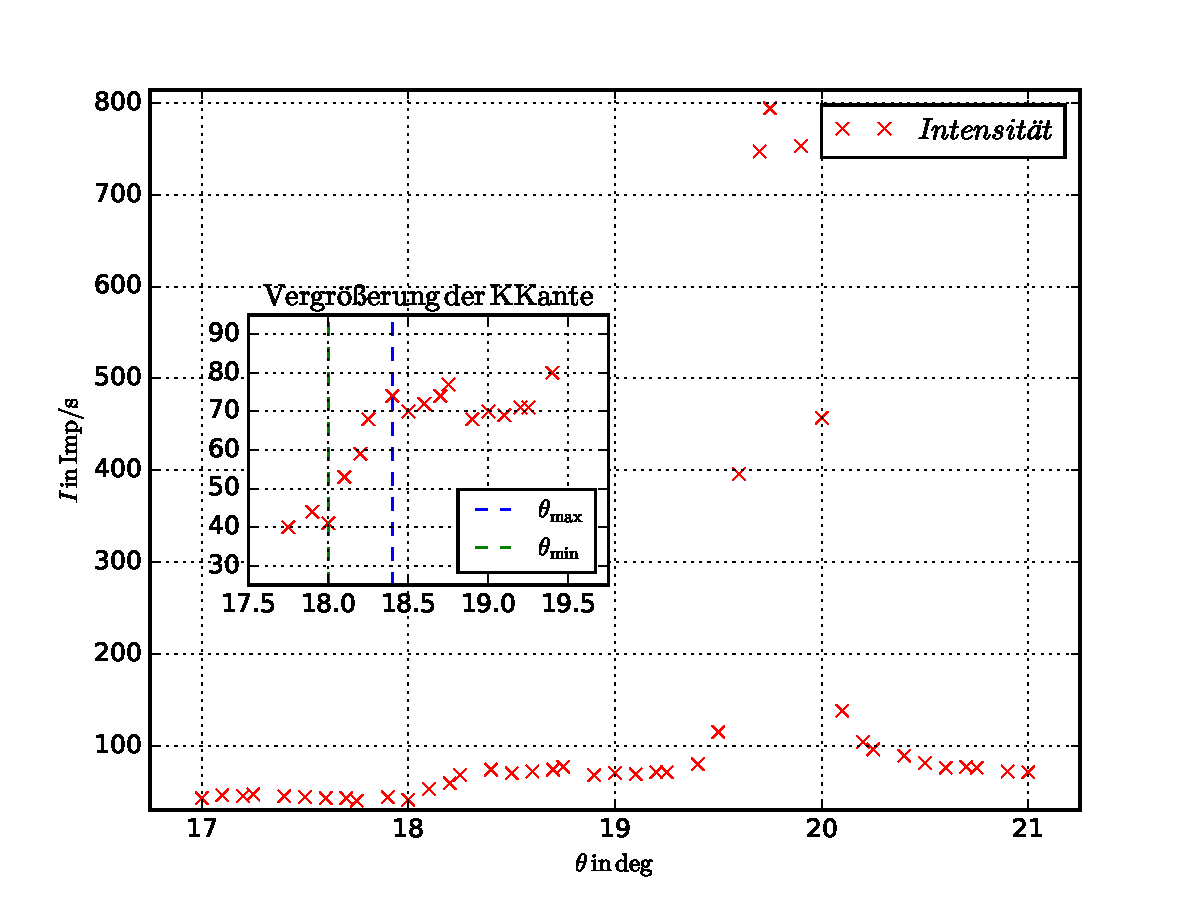
\includegraphics[width=1\textwidth]{../Messdaten/zink.pdf}
  \caption{Gemessenes Absorptionsspektrum für Zink. Zusätzlich ist in dem Plot eine Vergrößerung der K-Kante zu sehen.} %Hingegen passt nicht
  \label{fig: absotp_zink}
\end{figure}
In der Abbildung ist zusätzlich auch die beiden Winkel $\theta\ua{min}$ und $\theta\ua{max}$ die die K-Kante einschränken
eingezeichnet. Um die Energie der K-Kante zu bestimmen wird der Mittelwert der beiden Winekl bestimmt
\begin{equation}
  \label{eq:theta_k}
  \theta\ua{K}=\theta\ua{min}+\left(\theta\ua{max}-\theta\ua{min}\right)
\end{equation}
und anschließend mit Gleichung \eqref{} in die entsprechende Energie umgerechnet.
Für Zink ergibt sich als Energie der K-Kante
\begin{equation*}
  E\ua{K,zink}=\SI{9.9}{\kilo\eV} \quad \text{mit}\quad \theta\ua{min}=\SI{18.0}{\degree},\,\theta\ua{max}=\SI{18.4}{\degree}
\end{equation*}
Mit der Gleichung \eqref{} kann aus der Energien $E\ua{K}$ allgemein die Abschirmzahl
bestimmt werden.
Für Zink ergibt sich
\begin{equation}
  \label{eq: abschirm_zink}
  \sigma\ua{K}=3.1.
\end{equation}
\subsubsection{Untersuchung von $\ce{Ge}$,$\ce{Zr}$,$\ce{Br}$,$\ce{Sr}$}
Die für die einzelenen Elemente gemessenen Spektren sind in Abbildung \ref{fig: spektrum_brom_germanium} und
\ref{fig: spektrum_strontium_zirconium} dargestellt. Die zugehörogen Messwerte befinden sich in den Tabellen \ref{tab: zr}- \ref{tab: strom}.
\begin{figure}
  \centering
  \begin{subfigure}{0.48\textwidth}
    \centering
    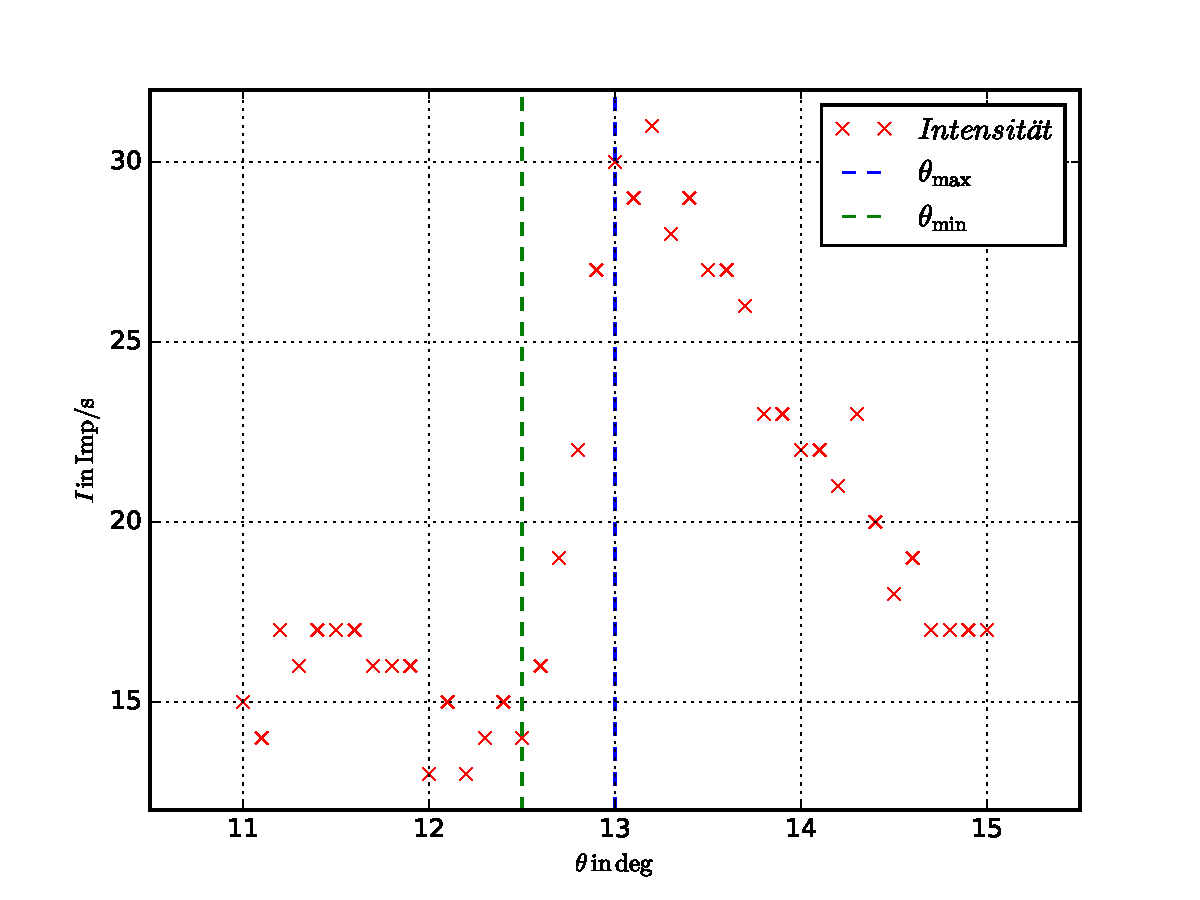
\includegraphics[width=1 \textwidth]{../Messdaten/brom.pdf}
    \caption{Gemessenes Spektrum für Brom $\ce{Br}$. Die zugehörigen Messwerte sind in Tabelle \ref{tab: brom} zu finden.} %der, geraden
    \label{fig: brom_spektrum}
  \end{subfigure}
  \begin{subfigure}{0.48\textwidth}
    \centering
    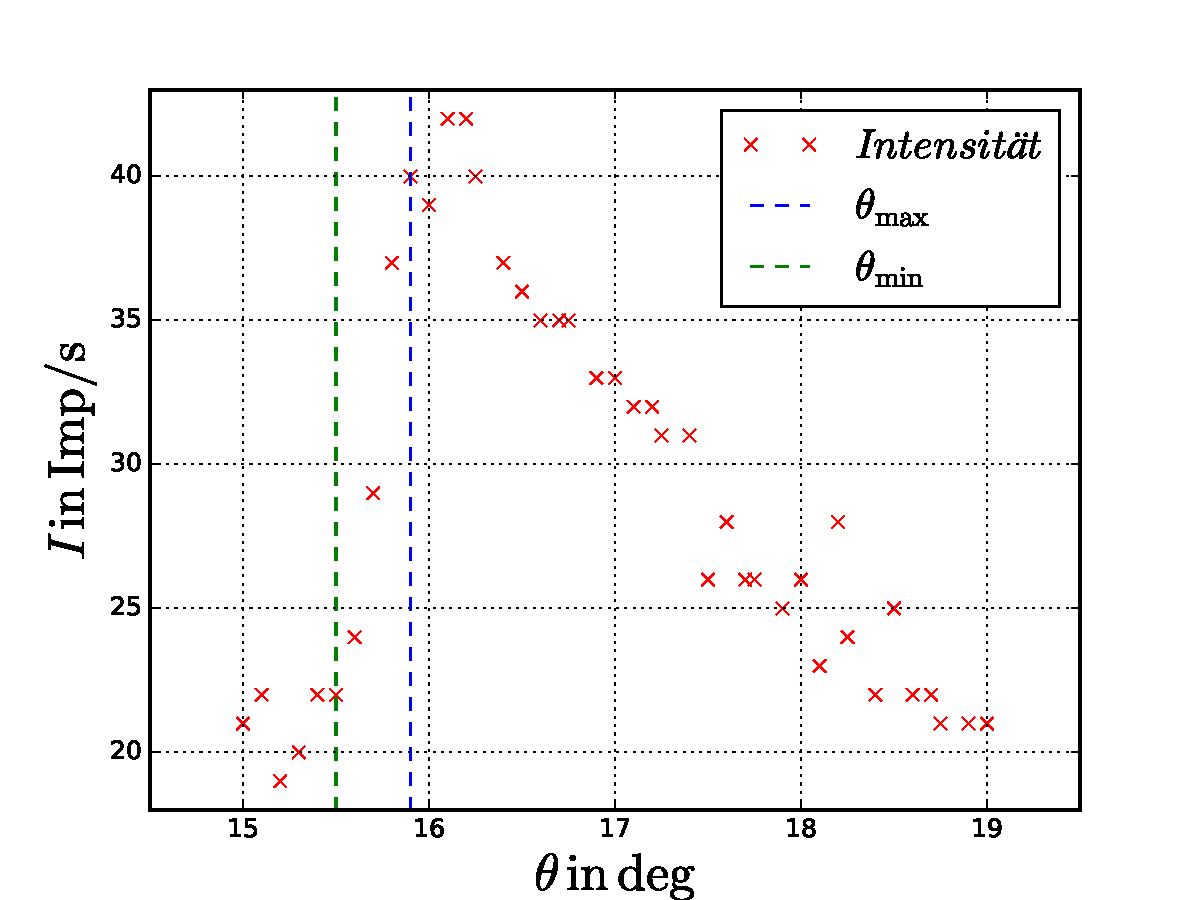
\includegraphics[width=1 \textwidth]{../Messdaten/germanium.pdf}
    \caption{Gemessenes Spektrum für Brom $\ce{Ge}$. Die zugehörigen Messwerte sind in Tabelle \ref{tab: germanium} zu finden.} %s.o.
    \label{fig: germaium_spektrum}
  \end{subfigure}
  \caption{Gemessene Absorptionsspektrum für Brom und Germanium.}
  \label{fig: spektrum_brom_germanium}
\end{figure}
\begin{figure}
  \centering
  \begin{subfigure}{0.48\textwidth}
    \centering
    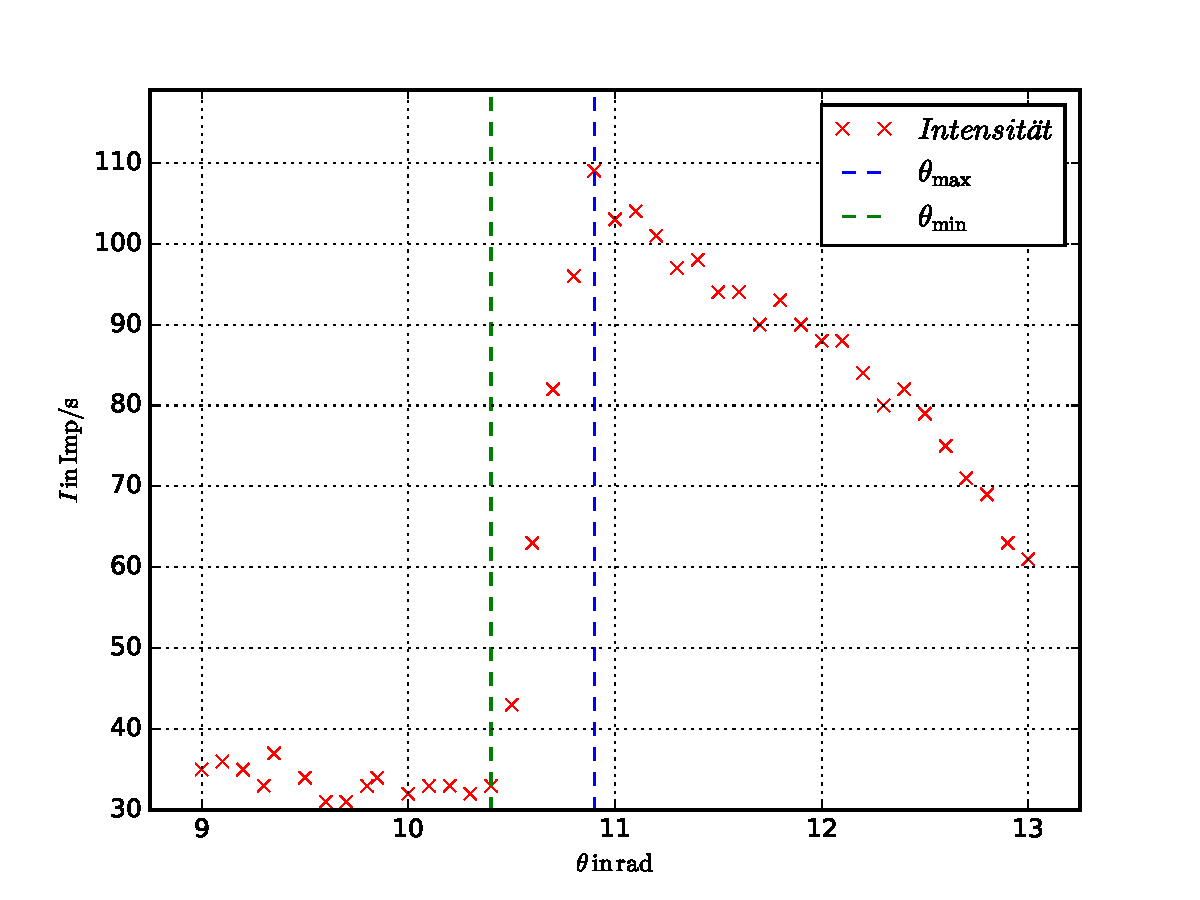
\includegraphics[width=1 \textwidth]{../Messdaten/strom.pdf}
    \caption{Gemessenes Spektrum für Strontium $\ce{Sr}$. Die zugehörigen Messwerte sind in Tabelle \ref{tab: strom} zu finden.}
    \label{fig: frank_hertz}
  \end{subfigure}
  \begin{subfigure}{0.48\textwidth}
    \centering
    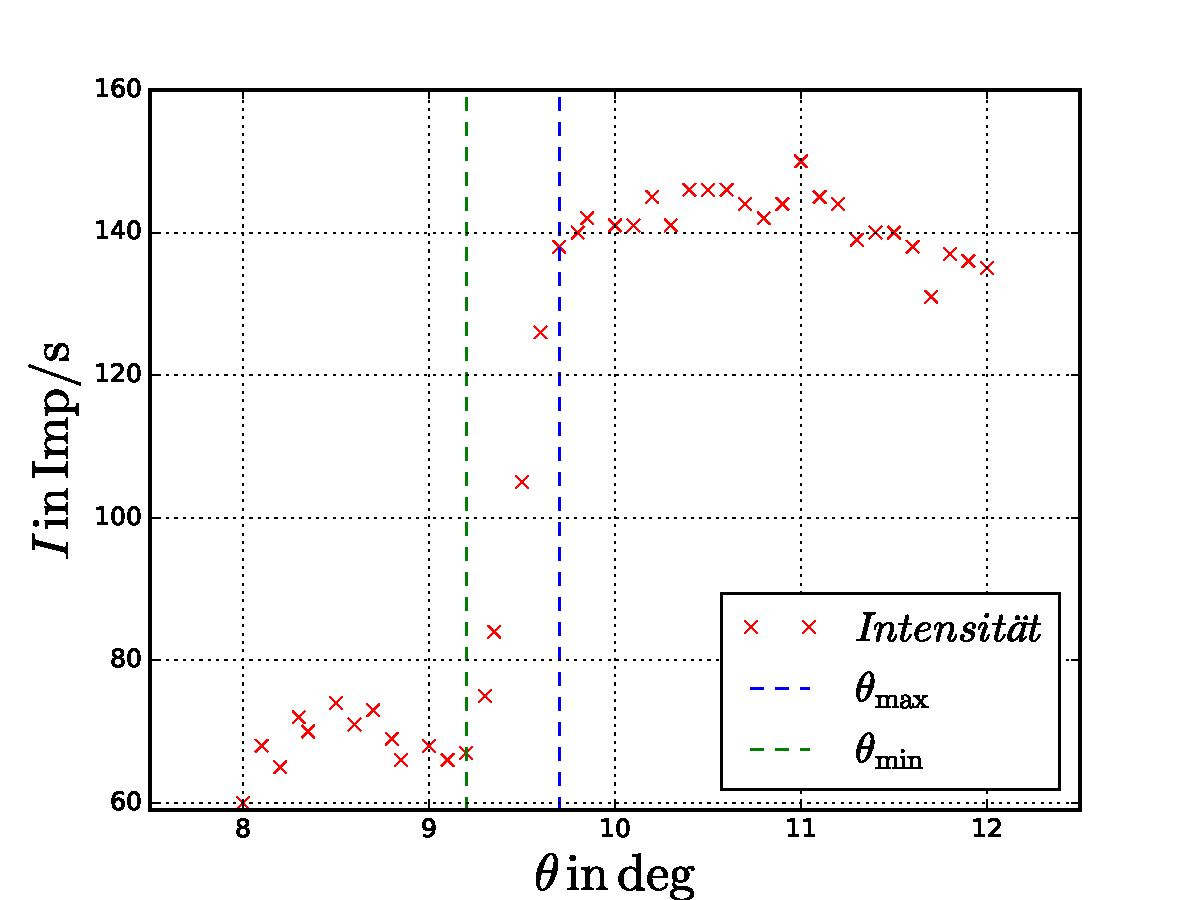
\includegraphics[width=1 \textwidth]{../Messdaten/zr.pdf}
    \caption{Gemessenes Spektrum für Zirconium $\ce{Zr}$. Die zugehörigen Messwerte sind in Tabelle \ref{tab: zr} zu finden.  } %s.o.
    \label{fig: enrgie_hot}
  \end{subfigure}
  \caption{Gemessene Absorptionsspektrum für Strontium und Zirconium.}
  \label{fig: spektrum_strontium_zirconium}
\end{figure}
Analog zu Kapitel \ref{sec: zink} werden die Enegerie $E\ua{K}$ und $\sigma\ua{K}$
bestimmt. Die sich Ergebnisse werden in Tabelle \ref{tab: messergebnisse} aufgeführt.
\begin{table}
  \centering
  \caption{Messergebnisse}
  \label{tab: messergebnisse}
  \begin{tabular}{S S S S S S}
    \toprule
    {Element}&   {$\theta\ua{min}$ in $\si{\degree}$ } & {$\theta\ua{max}$ in $\si{\degree}$} & {$E\ua{K}$ in $\si{\kilo\eV}$} &{$\sigma\ua{K}$}  \\
    \midrule
    $\ce{Zr}$ & 9.2 & 9.7 & 18.8 & 2.88\\
    $\ce{Ge}$  & 15.5 & 15.9 & 11.4 & 3.09\\
    $\ce{Br}$&  12.5 & 13.0 & 13.9 & 2.98 \\
    $\ce{Sr}$ & 10.4 & 10.9 & 16.7 & 3.01 \\
    \bottomrule
  \end{tabular}
\end{table}
\begin{table}
\centering
\caption{Messwerte bei der Untersuchung des Emmissionspektrum von $\ce{Zr}$.} 
\label{tab: zr}
\begin{tabular}{S S }
\toprule
{$\theta \, / \, \si{\degree}$} & {$I \, / \, \mathrm{Imp}/\mathrm{s}$}  \\
\midrule
 8.0  & 60.0\\
8.1  & 68.0\\
8.2  & 65.0\\
8.3  & 72.0\\
8.3  & 70.0\\
8.5  & 74.0\\
8.6  & 71.0\\
8.7  & 73.0\\
8.8  & 69.0\\
8.8  & 66.0\\
9.0  & 68.0\\
9.1  & 66.0\\
9.2  & 67.0\\
9.3  & 75.0\\
9.3  & 84.0\\
9.5  & 105.0\\
9.6  & 126.0\\
9.7  & 138.0\\
9.8  & 140.0\\
9.8  & 142.0\\
10.0  & 141.0\\
10.1  & 141.0\\
10.2  & 145.0\\
10.3  & 141.0\\
10.4  & 146.0\\
10.5  & 146.0\\
10.6  & 146.0\\
10.7  & 144.0\\
10.8  & 142.0\\
10.9  & 144.0\\
11.0  & 150.0\\
11.1  & 145.0\\
11.2  & 144.0\\
11.3  & 139.0\\
11.4  & 140.0\\
11.5  & 140.0\\
11.6  & 138.0\\
11.7  & 131.0\\
11.8  & 137.0\\
11.9  & 136.0\\
12.0  & 135.0\\
\bottomrule
\end{tabular}
\end{table}

\begin{table}
\centering
\caption{Messwerte bei der Untersuchung des Absorptionsspektrums von $\ce{Br}$.}
\label{tab: brom}
\begin{tabular}{S S S S }
\toprule
{$\theta \, / \, \si{\degree}$} & {$I \, / \, \mathrm{Imp}/\mathrm{s}$} & {$\theta \, / \, \si{\degree}$} & {$I \, / \, \mathrm{Imp}/\mathrm{s}$}  \\
\midrule
11.00  & 15& 13.10  &  29\\
11.10  & 14 & 13.20  & 31\\
11.20  & 17 & 13.30  & 28\\
11.30  & 16 & 13.40  & 29\\
11.40  & 17 & 13.50  & 27\\
11.50  & 17 & 13.60  & 27\\
11.60  & 17 & 13.70  & 26\\
11.70  & 16 & 13.80  & 23\\
11.80  & 16 & 13.90  & 23\\
11.90  & 16 & 14.00  & 22\\
12.00  & 13 & 14.10  & 22\\
12.10  & 15 & 14.20  & 21\\
12.20  & 13 & 14.30  & 23\\
12.30  & 14 & 14.40  & 20\\
12.40  & 15 & 14.50  & 18\\
12.50  & 14 & 14.60  & 19\\
12.60  & 16 & 14.70  & 17\\
12.70  & 19 & 14.80  & 17\\
12.80  & 22 & 14.90  & 17\\
12.90  & 27 & 15.00  & 17\\
13.00  & 30 & \,\,\text{-}   & \,\,\text{-} \\




















\bottomrule
\end{tabular}
\end{table}

\begin{table}
\centering
\caption{Messwerte bei der Untersuchung des Emmissionspektrum von $\ce{Ge}$.} 
\label{tab: germanium}
\begin{tabular}{S S }
\toprule
{$\theta \, / \, \si{\degree}$} & {$I \, / \, \mathrm{Imp}/\mathrm{s}$}  \\
\midrule
 15.0  & 21.0\\
15.1  & 22.0\\
15.2  & 19.0\\
15.3  & 20.0\\
15.4  & 22.0\\
15.5  & 22.0\\
15.6  & 24.0\\
15.7  & 29.0\\
15.8  & 37.0\\
15.9  & 40.0\\
16.0  & 39.0\\
16.1  & 42.0\\
16.2  & 42.0\\
16.2  & 40.0\\
16.4  & 37.0\\
16.5  & 36.0\\
16.6  & 35.0\\
16.7  & 35.0\\
16.8  & 35.0\\
16.9  & 33.0\\
17.0  & 33.0\\
17.1  & 32.0\\
17.2  & 32.0\\
17.2  & 31.0\\
17.4  & 31.0\\
17.5  & 26.0\\
17.6  & 28.0\\
17.7  & 26.0\\
17.8  & 26.0\\
17.9  & 25.0\\
18.0  & 26.0\\
18.1  & 23.0\\
18.2  & 28.0\\
18.2  & 24.0\\
18.4  & 22.0\\
18.5  & 25.0\\
18.6  & 22.0\\
18.7  & 22.0\\
18.8  & 21.0\\
18.9  & 21.0\\
19.0  & 21.0\\
\bottomrule
\end{tabular}
\end{table}

\begin{table}
\centering
\caption{Messwerte bei der Untersuchung des Emmissionspektrum von $\ce{Sr}$.}
\label{tab: strom}
\begin{tabular}{S S S S}
\toprule
{$\theta \, / \, \si{\degree}$} & {$I \, / \, \mathrm{Imp}/\mathrm{s}$} & {$\theta \, / \, \si{\degree}$} & {$I \, / \, \mathrm{Imp}/\mathrm{s}$}  \\
\midrule
9.00  & 35 & 11.10  & 104\\
9.10  & 36 & 11.20  & 101\\
9.20  & 35 & 11.30  & 97\\
9.30  & 33 & 11.40  & 98\\
9.35  & 37 & 11.50  & 94\\
9.50  & 34 & 11.60  & 94\\
9.60  & 31 & 11.70  & 90\\
9.70  & 31 & 11.80  & 93\\
9.80  & 33 & 11.90  & 90\\
9.85  & 34 & 12.00  & 88\\
10.00  & 32 & 12.10  & 88\\
10.10  & 33 &12.20  & 84\\
10.20  & 33 & 12.30  & 80\\
10.30  & 32 & 12.40  & 82\\
10.40  & 33 & 12.50  & 79\\
10.50  & 43 & 12.60  & 75\\
10.60  & 63 & 12.70  & 71\\
10.70  & 82 & 12.80  & 69\\
10.80  & 96 & 12.90  & 63\\
10.90  & 109 &13.00  & 61\\
11.00  & 103 & \,\,\text{-}  & \,\,\text{-} \\
\bottomrule
\end{tabular}
\end{table}


\subsubsection{Untersuchung des Absorptionsspektrum von Gold $\ce{Au}$}
Bei der Untersuchung der beiden L-Kanten ($L_2$ und $L_3$) wird die Apperatur, wie folgt
konfiguriert:
\begin{equation*}
  \theta\in\left[\theta\ua{\theta\ua{L_3}}-2,\ua{\theta\ua{L_2}}+2\right]\,\si{\degree},\quad \Delta\theta=\SI{0.1}{\degree}, \quad \Delta t=\SI{20}{\second}.
\end{equation*}
Dabei wurden die Winkel
\begin{equation*}
  \ua{\theta\ua{L_2}}=\SI{12.95}{\degree} \qquad  \ua{\theta\ua{L_3}}=\SI{14.95}{\degree}
\end{equation*}
aus der Literatur \cite{} notiert.
Die aufgenommenen Messwerte sind in Tabelle \ref{tab: gold} aufgelistet und in Abbildung
\ref{fig: absotp_gold} aufgetragen. In dieser sind die abgelesenen $L_2$ und $L_2$ Kanten eingezeichnet.
\begin{table}
\centering
\caption{Messwerte bei der Untersuchung des Emmissionspektrum von $\ce{Cu}$.}
\label{tab: gold}
\begin{tabular}{S S S S }
\toprule
{$\theta \, / \, \si{\degree}$} & {$I \, / \, \mathrm{Imp}/\mathrm{s}$} & {$\theta \, / \, \si{\degree}$} & {$I \, / \, \mathrm{Imp}/\mathrm{s}$}  \\
\midrule
 11.0  & 79  & 14.1  & 56\\
11.1  & 81  & 14.2  & 60\\
11.2  & 80  & 14.3  & 53\\
11.3  & 77  & 14.4  & 56\\
11.4  & 80  & 14.5  & 60\\
11.5  & 75  & 14.6  & 66\\
11.6  & 72  & 14.7  & 73\\
11.7  & 72  & 14.8  & 75\\
11.8  & 74  & 14.9  & 84\\
11.9  & 72  & 15.0  & 73\\
12.0  & 76  & 15.1  & 77\\
12.1  & 75  & 15.2  & 76\\
12.2  & 75  & 15.3  & 75\\
12.3  & 77  & 15.4  & 76\\
12.4  & 78  & 15.5  & 72\\
12.5  & 75  & 15.6  & 70\\
12.6  & 80  & 15.7  & 69\\
12.7  & 85  & 15.8  & 67\\
12.8  & 82  & 15.9  & 65\\
12.9  & 77  & 16.0  & 64\\
13.0  & 74  & 16.1  & 63\\
13.1  & 71  & 16.2  & 61\\
13.2  & 69  & 16.2  & 58\\
13.3  & 67  & 16.4  & 59\\
13.4  & 62  & 16.5  & 60\\
13.5  & 63  & 16.6  & 58\\
13.6  & 63  & 16.7  & 58\\
13.7  & 59  & 16.8  & 56\\
13.8  & 57  & 16.9  & 54\\
13.9  & 58  & 17.0  & 55\\
14.0  & 59  & \,\,\text{-}  & \,\,\text{-}\\ 
\bottomrule
\end{tabular}
\end{table}

\begin{figure}
  \centering
  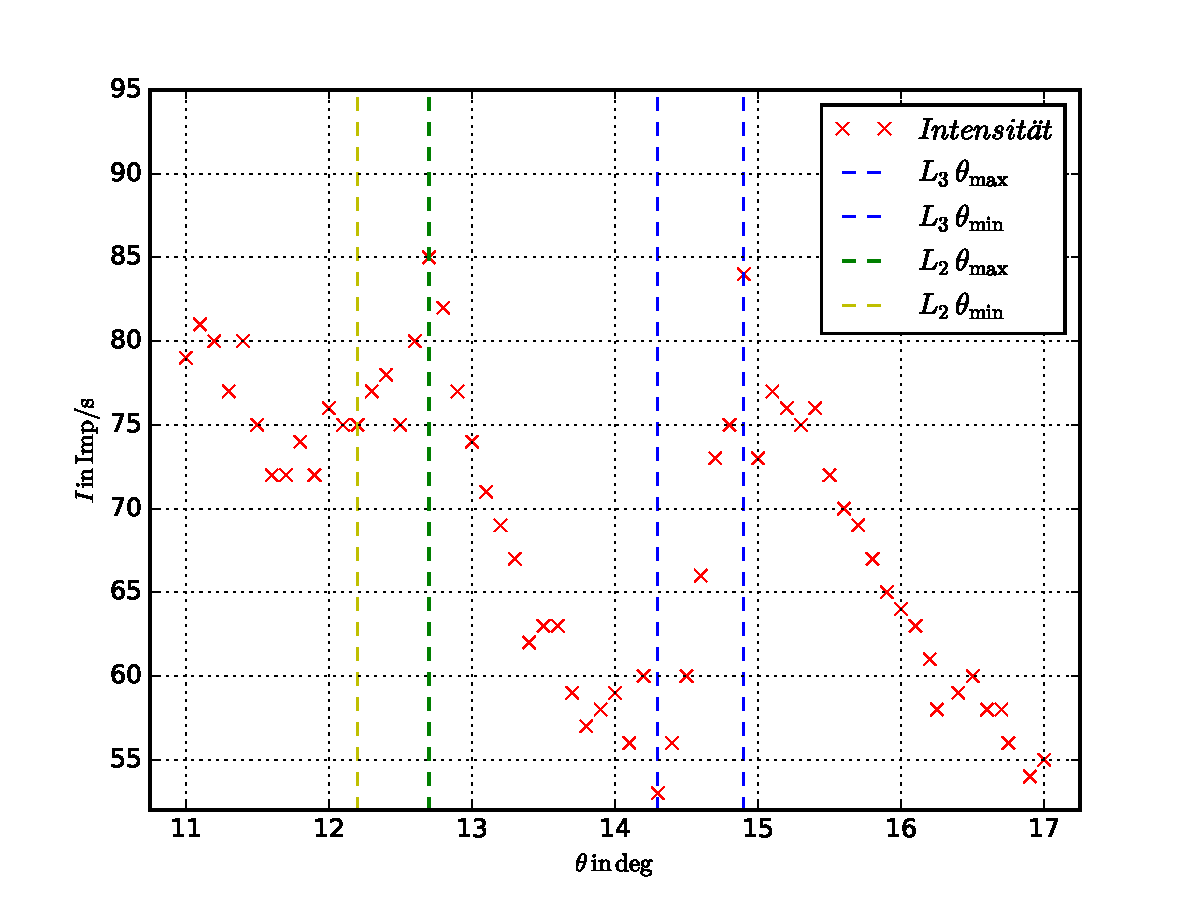
\includegraphics[width=0.8\textwidth]{../Messdaten/gold.pdf}
  \caption{Gemessenes Absorptionsspektrum für Gold. In der Graphik sind die abgelesenen $L_2$ und $L_2$ Kanten farblich markiert.} %Hingegen passt nicht
  \label{fig: absotp_gold}
\end{figure}
Die abgelesenen Winkel werden mit Gleichung \eqref{} auf die Energie umgerechnet:
\begin{equation}
  \label{eq:l_kanten_gold}
  E\ua{L_2}=\SI{14.0}{\kilo\eV}  \qquad   E\ua{L_3}=\SI{12.0}{\kilo\eV}.
\end{equation}
Mit den Energiewerten und der Kernladungszahl $Z\ua{Au}=79$ kann die Abschirmkonstante
von Gold bestimmt werden. Unter Verwendung von Gleichung \eqref{} ergibt sich
\begin{equation*}
    \sigma\ua{L}=1.7.
\end{equation*}

\subsection{Bestimmung der Rydbergenergie}
Für die Bestimmung Rydbergenerigie $R_\infty$ wird durch die zuvor
bestimmten Energien $E\ua{K}$ eine Regeressionsgerade der Form
\begin{equation*}
  g(x)=mx+b=
\end{equation*}
gelegt. Mit der Ausgleichsrechnung sollen die Parameter der Gleichung \eqref{}
bestimmt werden. Beim Koeffizientenvergleich ergibt sich das die Rydberggenergie
gerade
\begin{equation*}
  R_\infty=m^2
\end{equation*}
ist.
Die Energien sind in Tabelle \ref{tab: ener_ryd} gelistet
und in der Abbildung \ref{fig: ryd_ener} gezeichnet. In der Abbildung ist
die resultierende Regressionsgerade mit aufgetragen.
\begin{table}
\centering
\caption{Experimentell bestimmten Energie $E_{\mathrm{K}}$}
\label{tab: ener_ryd}
\begin{tabular}{S S S}
\toprule
{Element} & {Z} & {$E_{\mathrm{K}}$}  \\
\midrule
$\ce{Zr}$& 40  & 136.9\\ 
$\ce{Ge}$ & 32  & 106.7\\
$\ce{Br}$ &35  & 118.1\\
$\ce{Sr}$ &38  & 129.1\\
 $\ce{Zn}$ &30  & 99.3\\
\bottomrule
\end{tabular}
\end{table}

\begin{figure}
  \centering
  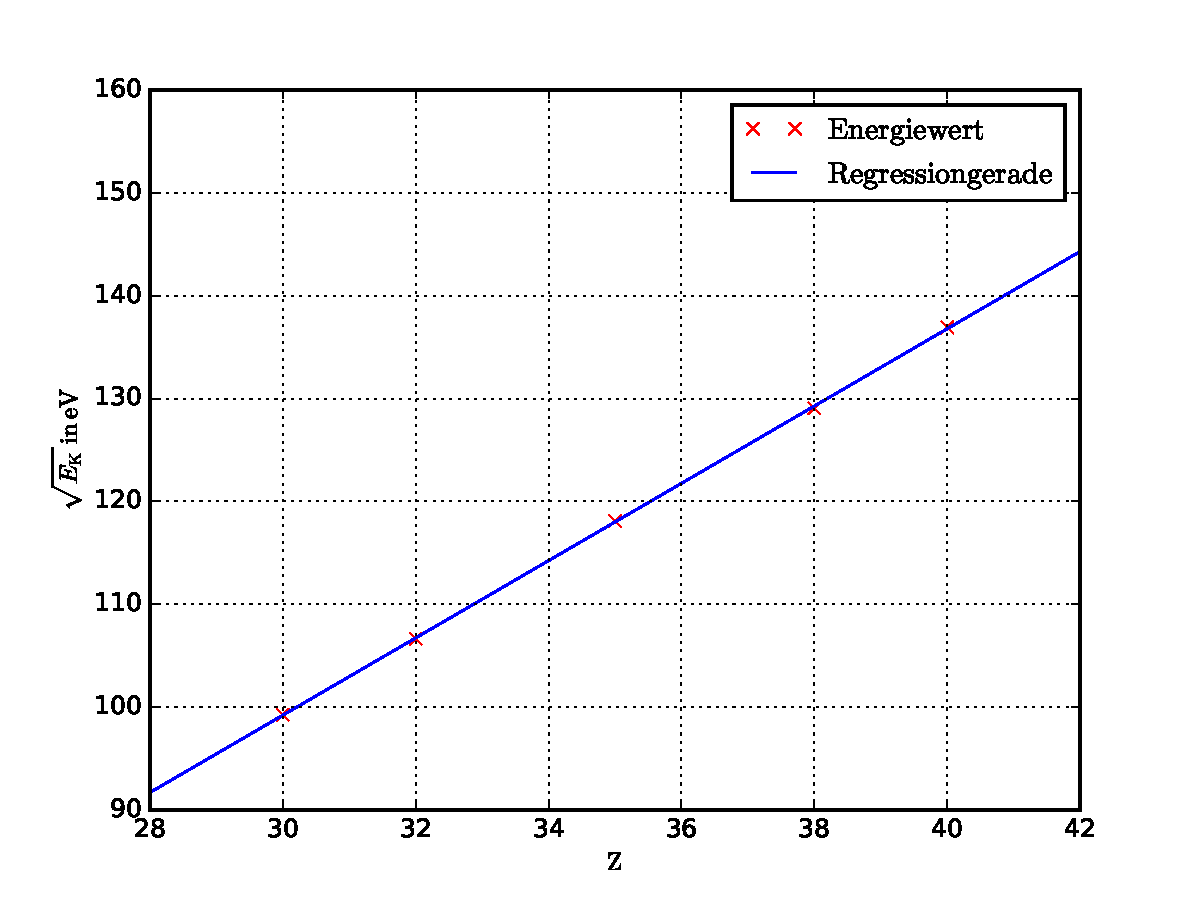
\includegraphics[width=0.7\textwidth]{../Messdaten/energie_z.pdf}
  \caption{Auftagung der experimentell berechneten Energien $E\ua{K}$ gegen die Kernladungszahl $Z$. Zusätzlich ist in der Abbildung die zugehöroge Ausgleichsgerade zu sehen. } %Hingegen passt nicht
  \label{fig: ryd_ener}
\end{figure}
Die Ausgleichsrechnung liefert folgende Parameter:
\begin{equation*}
m=\num{3.76\pm0.02}\,\sqrt{\si{\eV}} \qquad b=\num{-13.5\pm0.7}\,\sqrt{\si{\eV}}.
\end{equation*}
Damit wird die Rydbergenergie bestimmt zu:
\begin{equation}
  R_\infty=\SI{14.11\pm0.15}{\eV}
\end{equation}
